\section{Research}
\label{sec:research}


\subsection{Introduction}
\label{sec:introduction}

% Automated Vehicles are introduced (in Singapore)
The development of automated vehicles (AVs) has made significant progress. It is expected that before 2020, automated and autonomous vehicles will be introduced in controlled environments, whereas autonomous vehicles will be mainstream by 2040 \cite{madni2018autonomous} or earlier \cite{bimbraw2015autonomous}. Especially in densely populated cities such as Singapore, there is a need for automated vehicles to increase traffic safety and traffic efficiency by enabling flexible, automated, mobility-on-demand systems \cite{spieser2014toward}, scheduled services for public transport needs, and automated freight and service vehicles to support 24 hours operations and labor shortage needs.

% Assessment of AVs is important
An important aspect in the development of AVs is the safety assessment of the AVs \cite{bengler2014threedecades, stellet2015taxonomy, putz2017pegasus, wachenfeld2016release}. For legal and public acceptance of AVs, a clear definition of system performance is important, as are quantitative measures for the system quality. The more traditional methods \cite{ISO26262, response2006code}, used for evaluation of driver assistance systems, are no longer sufficient for assessment of the safety of higher level AVs, as it is not feasible to complete the quantity of testing required by these methodologies \cite{wachenfeld2016release}. Therefore, the development of assessment methods is important to not delay the deployment of AVs \cite{bengler2014threedecades}.

% Scenario-based approach
One proposed way to assess safety is to test drive AVs in real traffic, observe their performance, and make statistical comparisons to human driver performance. However, this requires AVs to drive hundreds of millions of kilometers and sometimes hundreds of billions of kilometers to demonstrate their reliability in terms of fatalities and injuries \cite{kalra2016driving}. It does not seem to be feasible to drive these millions of kilometers with the increased speed of development of automated driving (AD) functions and the high level of safety requirements that are expected from these functions. As an alternative, a scenario-based assessment is adopted \cite{putz2017pegasus, stellet2015taxonomy, deGelder2017assessment, ploeg2018cetran, elrofai2018scenario}. 
% Scenarios are obtained with data
These test-scenarios can be knowledge-driven or data-driven \cite{stellet2015taxonomy}. A drawback of knowledge-based test scenarios is that it does not allow to generalize the results to the performance of the system-under-test when operating in traffic, i.e., the test cases may not be valid or representative for real-world traffic. A data-driven approach is adopted, as it allows to generalize the results \cite{deGelder2017assessment}. The challenge is, however, to extract the interesting, e.g., performance critical, scenarios from the data, such that the number of simulations is still limited.

\subsection{Focus of research}
\label{sec:focus}

\Cref{fig:scheme} presents a schematic overview of the process of the assessment of an automated vehicle using real-world driving data. The primary goal of the research is to develop a methodology for the generation of the test cases using the preprocessed data, represented by the green blocks in \cref{fig:scheme}. This is achieved by detecting and parameterizing so-called activities. Using the activities and the static environment, the scenarios can be obtained, after which test cases can be generated for the assessment of the AV.

\tikzstyle{block}=[node distance=5.2em, text width=4.5em, minimum height=7em, align=center, rounded corners=8pt, font=\small]
\tikzstyle{my brace}=[decorate, decoration={brace, amplitude=10pt}]
\tikzstyle{horz}=[node distance=2.7em]
\tikzstyle{vert}=[node distance=4em]
\begin{figure}[b]
	\centering
	\begin{tikzpicture}[scale=0.95, every node/.style={transform shape}]
		% Draw the blocks
		\node[block, fill=blue!30](dc){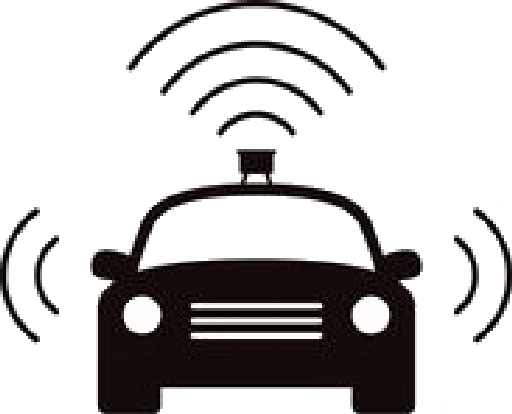
\includegraphics[width=4em]{data_collection.png} \\ Data collection};
		\node[block, fill=blue!30, right of=dc](dp){
\includegraphics[width=2.5em]{data_processing.png} \\ Data preprocessing};
		\node[block, fill=green!30, right of=dp](ed){
\includegraphics[width=4.2em]{event_detection.png} \\ Activity detection};
		\node[block, fill=green!30, right of=ed](s){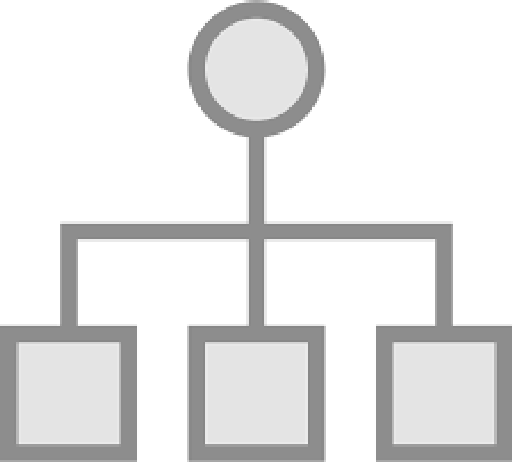
\includegraphics[width=3em]{scenario_mining.png} \\ Scenario mining};
		\node[block, fill=green!30, right of=s](p){
\includegraphics[width=3em]{parametrisation.png} \\ Parame-trization};
		\node[block, fill=green!30, right of=p](tc){
\includegraphics[width=3.2em]{scenarios.png} \\ Test case genera-tion};
		\node[block, fill=red!30, right of=tc](sim){
\includegraphics[width=4em]{simulation.png} \\ Simulation};
		\node[block, fill=red!30, right of=sim](eval){
\includegraphics[width=3em]{evaluation.png} \\ Evaluation};
		
		% Show completeness part
		\node[horz, left of=ed](b1){};
		\node[vert, below of=b1](b2){};
		\node[horz, right of=tc](b3){};
		\node[vert, below of=b3](b4){};
		\draw[my brace](b4) -- (b2) node[midway, yshift=-2em, align=center]{Completeness};
	\end{tikzpicture}
	\vspace{-1em}
	\caption{Schematic overview of the process of the assessment of an automated vehicle using real-world data. The green blocks are the focus of the PhD research.}
	\label{fig:scheme}
\end{figure}


First of all, a clear definition of scenario is required to avoid the ambiguity that often arises when talking about \emph{scenarios}. Next to that, related notions need to be defined, e.g., the components that constitute a scenario, such as the activities and the static environment. 

% Activity detection
An activity is considered the smallest building block of the dynamic part of the scenario (maneuver of the ego vehicle and the dynamic environment). An activity refers to the behavior of an actor, such as ``braking'' and ``changing lane''. The first step is to detect the activities from the preprocessed data. 

% Scenario mining
In scenario mining, the events and activities that are independently identified for the ego vehicle, the other traffic participants, the static environment, and the conditions are combined to construct a scenario. 

% Parametrization
The recorded scenarios (and its associated activities) are to be stored in a database \cite{elrofai2018scenario}. The scenario database does not contain raw sensor data, but a parametrized model of the real world based on the sensor signals. Therefore, dependency of the stored scenarios on the sensor set with which the scenario was recorded is avoided. The fact that the stored scenarios do not contain the original sensor data brings several benefits. 
\begin{itemize}
	\item The original sensor data might be sensitive as it reveals the sensor setup and processing capabilities of a car. This is much less of an issue when only parameters of the models of the scenarios are stored. Whereas the original sensor data is unlikely to be shared among different parties, the resulting scenarios might be shared, such that the involved parties can benefit from each other.
	\item By condensing the information of all sensors into the least amount of parameters that describe the scenario within the error bounds of sensors, substantial reduction in storage volume is achieved.
	\item All the parameters of scenarios of a specific scenario class can be used to construct probability density functions. These probability density functions can be used to generate test cases that lead to probabilistic results \cite{deGelder2017assessment}. Furthermore, it is possible, using the parametrized scenarios, to emphasize scenarios in which the system-under-test shows performance-critical behavior without a-priori knowledge of what scenarios might be critical \cite{deGelder2017assessment}. 
	\item The parametrized models of the scenarios allow for time interpolation. Hence, the stored scenarios can be used for any given sample time, regardless of the sample time of the original sensor data. 
\end{itemize}

% Test case generation

% Completeness


\subsection{Preliminary results}
\label{sec:results}

I mainly worked on defining an appropriate ontology regarding scenarios and quantifying completeness. 

\subsubsection{Ontology of scenario for the assessment of automated vehicles}
\label{sec:ontology}

The notion of scenario is frequently used in the context of automated driving \cite{putz2017pegasus, roesener2017comprehensive, gietelink2006development, hulshof2013autonomous, karaduman2013interactivebehavior, englund2016grand, xu2002effects, ebner2011identifying, ploeg2017GCDC, zofka2015datadrivetrafficscenarios}, despite the fact that an explicit definition is often not provided. However, as mentioned by various authors \cite{stellet2015taxonomy, alvarez2017prospective, zofka2015datadrivetrafficscenarios, aparicio2013pre, lesemann2011test, putz2017pegasus, geyer2014, ulbrich2015}, using a scenario in the context of the development or assessment of AVs requires a clear definition of a scenario. To this end, few definitions of a scenario in the context of (automated) driving have been proposed \cite{geyer2014, ulbrich2015, elrofai2016scenario}. For the context of the scenario database that we aim for \cite{elrofai2018scenario}, however, a more concrete definition of a scenario is required to minimize any ambiguity regarding the scenarios. Ultimately, an ontology is desired to directly use the definitions for the scenario database.

Part of the ontology are the definitions of the different concepts that are adopted. For defining the notion of a scenario, the following characteristics are considered:
\begin{enumerate}
	\item A scenario corresponds to a time interval \cite{go2004blind, geyer2014, ulbrich2015, elrofai2016scenario}.
	\item A scenario consists of one or several events \cite{vannotten2003updated, go2004blind, geyer2014, ulbrich2015, kahn1962, englund2016grand, schoemaker1993multiple, cuppens2002alert, bach2016modelbased}.
	\item Real-world traffic scenarios are quantitative scenarios.
	\item The time interval of a scenario contains all relevant events \cite{geyer2014}.
	\item A scenario can contain goal(s) of one or multiple actors \cite{geyer2014, ulbrich2015, elrofai2016scenario}.
	\item A scenario includes the description of the environment \cite{geyer2014, ulbrich2015, elrofai2016scenario, ebner2011identifying, schuldt2013effiziente, althoff2017CommonRoad}.
\end{enumerate}

Hence, a scenario is defined as follows.
\begin{definition}[Scenario]\label{def:scenario}
	A scenario is a quantitative description of the ego vehicle, its activities and/or goals, its dynamic environment (consisting of traffic environment and conditions) and its static environment. From the perspective of the ego vehicle, a scenario contains all relevant events.
\end{definition}

For the ontology, the other notions, such as ego vehicle, activity, dynamic environment, static environment, conditions, and events, need to be defined as well. However, this is out fo scope for this report.

Although a scenario is a quantitative description, there also exists a qualitative description of a scenario. We refer to the qualitative description of a scenario as a \emph{scenario class}. The qualitative description can be regarded as an abstraction of the quantitative scenario.

Scenarios are instances of scenario classes. A scenario class can contain multiple scenarios. On the other hand, a scenario may belong to one or multiple scenario classes. As an example, consider the scenario class ``Day'', which contains all scenarios that occur during the day, and the scenario class ``Rain'', which contains all scenarios with rain, see \cref{fig:venn diagram scenario class}. A scenario that occurs during the night without rain does not belong to any of the previously defined scenario classes. Likewise, a scenario that occurs during the day with rain belongs to both scenario classes ``Day'' and ``Rain''. 

\setlength{\venncircle}{10em}
\begin{figure}
	\centering
	\begin{tikzpicture}
		\fill[red, fill opacity=0.5] (-\venncircle/2, 0) circle (\venncircle);
		\fill[green, fill opacity=0.5] (\venncircle/2, 0) circle (\venncircle);
		\draw (-\venncircle/2, 0) circle (\venncircle);
		\draw (\venncircle/2, 0) circle (\venncircle);
		
		\node[anchor=east](daylight) at (-4/3*\venncircle, 3/4*\venncircle) {Day};
		\draw (daylight) -- ({(-sqrt(3)/2-1/2)*\venncircle}, \venncircle/2);
		\node[anchor=west](rain) at (4/3*\venncircle, 3/4*\venncircle) {Rain};
		\draw (rain) -- ({(sqrt(3)/2+1/2)*\venncircle}, \venncircle/2);
		
		\node[text width=\venncircle, align=center] at (-\venncircle, 0) {Scenarios without rain during day};
		\node[text width=\venncircle, align=center] at (0, 0) {Scenarios with rain during day};
		\node[text width=\venncircle, align=center] at (\venncircle, 0) {Scenarios with rain during night};
	\end{tikzpicture}
	\caption{The two circles correspond to the two scenario classes ``Day'' and ``Rain'', respectively. Scenarios that occur during the day with rain belong to both scenario classes ``Day'' and ``Rain''. The new scenario class ``Day and rain'' can be defined as the class that contains all scenarios that occur during the day with rain. The scenario class ``Day and rain'' is a subclass of the scenario classes ``Day'' and ``Rain''.}
	\label{fig:venn diagram scenario class}
\end{figure}

A scenario class can be a subclass of another scenario class. For example, when we continue our previous example and consider the scenario class ``Day and rain'', this scenario class is a subclass of the scenario classes ``Day'' and ``Rain''. Also, a scenario that occurs during the day with rain now belongs to three scenario classes: ``Day'', ``Rain'', and ``Day and rain''.

\subsubsection{Quantification of completeness}

To draw conclusions on how an AV would perform in real-world traffic, it is necessary to know how representative the scenario database, that is used for the scenario-based assessment of the AV, is. Therefore, it is important to quantify how complete the scenario database is \cite{geyer2014, alvarez2017prospective, stellet2015taxonomy}. To quantify how complete a scenario database is, it is assumed that a scenario is defined according to \cref{def:scenario} and that a scenario class refers to a qualitative description of a scenario, such as described in \cref{sec:ontology}. The problem of quantifying the completeness can now be divided into two subproblems.

\begin{itemize}
	\item The first subproblem deals with the quantification of the completeness regarding the number of scenario classes. 
	\item The second subproblem deals with the quantification of the completeness regarding the scenarios of a specific scenario class.
\end{itemize}

During my research, I only focused on the second subproblem. To address this problem, it is assumed that each scenario of a specific scenario class can be parametrized using similar variables. Therefore, a probability density function (pdf) can be estimated based on the recorded scenarios. This pdf can be used to generate new instances that serve as test cases for the assessment of AVs. To obtain test cases that reflect the real-world traffic, the estimated pdf needs to resemble the true underlying pdf. Therefore, the second subproblem is addressed by quantifying the uncertainty of the estimated pdf.

One way to estimate the uncertainty of an estimated pdf employs the so-called Mean Integrated Squared Error. Let $x \in \mathbb{R}^d$ be the vector of parameters and $f(x)$ the true underlying distribution. The pdf $f(x)$ is estimated using $n$ datapoints. Let $\hat{f}(x;n)$ denote the estimated pdf. This the MISE is defined as follows:
\begin{equation} \label{eq:mise}
	\mise{n} = \expectation{ \int_{\mathbb{R}^d} \left(\hat{f}(x;n) - f(x)\right)^2 \, \textup{d}x} = \int_{\mathbb{R}^d} \expectation{\left(\hat{f}(x;n) - f(x)\right)^2} \, \textup{d}x,
\end{equation}

For calculating the MISE, the true pdf $f(x)$ is required. However, the MISE can be estimated using $\hat{f}(x, n)$. When $f(x)$ is estimated using a parametric statistics, e.g., a Gaussian distribution, the posterior distributions of the parameters of the pdf can be used \cite{bishop2006pattern}, whereas for nonparametric statistics, e.g., Kernel Density Estimation \cite{rosenblatt1956remarks, parzen1962estimation}, the asymptotic MISE can be employed \cite{chen2017tutorial}. As this report is meant to give an overview of the research, more details on quantifying the completeness are omitted in this report.

\subsection{Papers and reports}
\label{sec:paper}

During last year, several papers and reports are written, among which is the following:
\begin{itemize}
	\item Paper on ontology for the Intelligent Vehicles Symposium (IV).
	\item Paper for ITS AP
	\item Report on scenario classes.
	\item Position paper of StreetWise.
\end{itemize}

\subsection{Outlook}
\label{sec:outlook}

Major
\begin{itemize}
	\item Paper on ontology
	\item Paper on completeness
	\item Overall paper describing the assessment procedure. Work out whole pipeline (including completeness, simulation) for at least one scenario class.
	\item Test case generation (including parametrization and estimation pdf)
\end{itemize}

Minor
\begin{itemize}
	\item Publish data
	\item Risk of a scenario class
	\item Detection/classification of activities.
\end{itemize}

Note: scenario mining already addressed by other people.
